\documentclass{article}
\usepackage[scale=.9]{geometry}
\usepackage{tikz}
\usetikzlibrary{
  spath3,
  intersections,
  hobby,
  external,
  decorations.pathreplacing,
  shapes.geometric,
}

\tikzset{
  external/figure name=knot,
  external/prefix=knotdiagrams/new-,
  external/system call={pdflatex \tikzexternalcheckshellescape -halt-on-error -interaction=batchmode -jobname "\image" "\texsource" && pdftoppm -png -singlefile "\image.pdf" "\image"},
}

\tikzexternalize
%\tikzset{external/force remake=true}

\let\origtikzsetnextfilename\tikzsetnextfilename
\def\tikzsetnextfilename#1{%
  \origtikzsetnextfilename{#1}%
  \mysetlabel{#1}%
}

\newcommand{\mysetlabel}[1]{%
  \gdef\mynextlabel{#1}}

\newcommand{\autolabel}{%
  \label{fig:\mynextlabel}
  \global\let\mynextlabel\relax
}


\tikzset{
  use Hobby shortcut,
  every picture/.style={
    execute at end picture={%
      \path ([shift={(-5pt,-5pt)}]current bounding box.south west)   ([shift={(5pt,5pt)}]current bounding box.north east);
    }
  },
  every spath component/.style={ultra thick, draw, red},
%  every trefoil component/.style={ultra thick, draw, red},
}

\begin{document}
\begin{figure}
\tikzsetnextfilename{unknot}
\centering
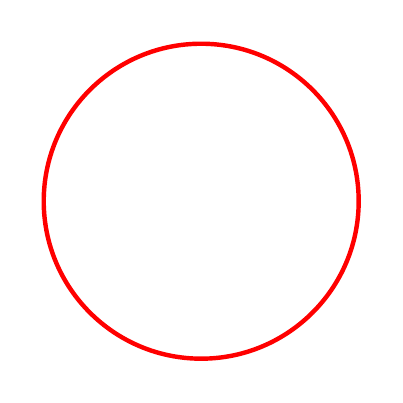
\begin{tikzpicture}
\draw[ultra thick,red] (0,0) circle[radius=2cm];
\end{tikzpicture}
\caption{Unknot}
\autolabel
\end{figure}

\begin{figure}
%% Trefoil
%\tikzset{external/export next=false}
\tikzsetnextfilename{trefoil}
\centering
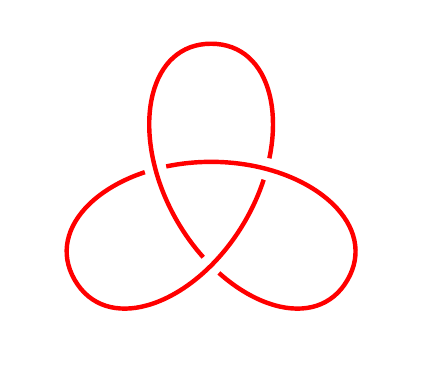
\begin{tikzpicture}
\path[spath/save=trefoil] ([closed]90:2) foreach \k in {1,...,3} { .. (-30+\k*240:.5) .. (90+\k*240:2) } (90:2);
\tikzset{
  spath/knot={trefoil}{8pt}{1,3,5},
}
\end{tikzpicture}
\caption{Trefoil}
\autolabel
\end{figure}

\begin{figure}
%% Figure 8
\tikzsetnextfilename{figure8}
%\tikzset{external/export next=false}
\centering

\begin{tikzpicture}
\path[spath/save=figure8] ([closed]0,0) .. (1.5,1) .. (.5,2) .. (-.5,1) .. (.5,0) .. (0,-.5) .. (-.5,0) .. (.5,1) .. (-.5,2) .. (-1.5,1) .. (0,0);
\tikzset{spath/knot={figure8}{8pt}{2,4,6,8}}
\path (0,-.7);
\end{tikzpicture}
\caption{Figure 8}
\autolabel
\end{figure}

\begin{figure}
%% Cinquefoil
\centering
\tikzsetnextfilename{cinquefoil}
%\tikzset{external/export next=false}
%\tikzset{external/force remake}
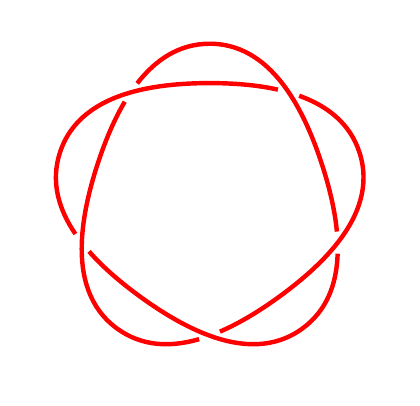
\begin{tikzpicture}
\path[spath/save=cinquefoil] ([closed]90:2) foreach \k in {1,...,5} { .. (18+\k*144:1.5) .. (90+\k*144:2) } (90:2);
\tikzset{spath/knot={cinquefoil}{8pt}{2,4,6,8,10}}
\end{tikzpicture}
\caption{Cinquefoil}
\autolabel
\end{figure}

\begin{figure}
%% 5_2
\centering
\tikzsetnextfilename{5-2}
%\tikzset{external/export next=false}
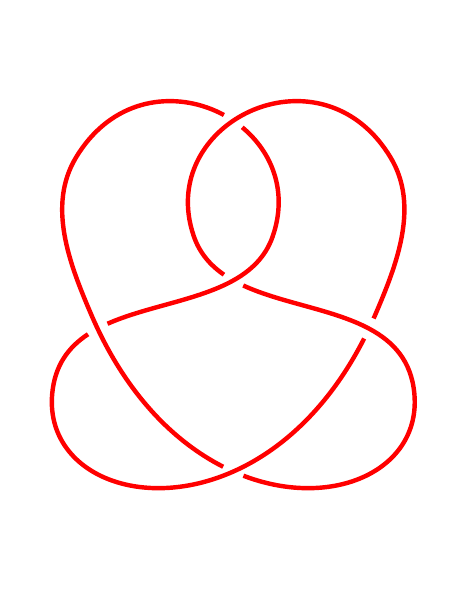
\begin{tikzpicture}
\path[spath/save=5-2] ([closed]2,2) .. (1.8,0) .. (-2.3,-1) .. (.5,1) .. (-2,2) .. (-1.8,0) .. (2.3,-1) .. (-.5,1) .. (2,2);
\tikzset{spath/knot={5-2}{8pt}{2,4,...,10}}
\end{tikzpicture}
\caption{\(5_2\)}
\autolabel
\end{figure}

\begin{figure}
%% 6_1
\centering
\tikzsetnextfilename{6-1}
%\tikzset{external/export next=false}
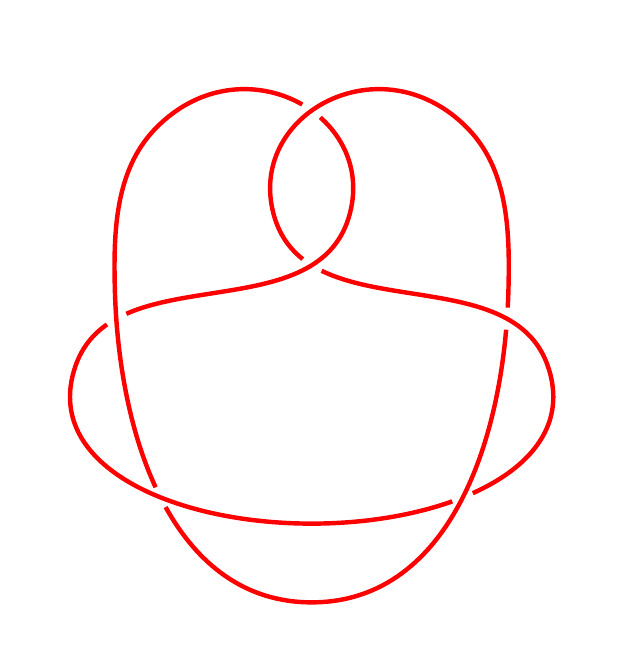
\begin{tikzpicture}
\path[spath/save=6-1] ([closed]2,2) .. (2.5,0) .. (0,-4) .. (-2.5,0) .. (-2,2) .. (.5,1) .. (-3,-1) .. (0,-3) .. (3,-1) .. (-.5,1) .. (2,2);
\tikzset{spath/knot={6-1}{8pt}{2,4,...,12}}
\end{tikzpicture}
\caption{\(6_1\)}
\autolabel
\end{figure}

\begin{figure}
%% 6_2
\centering
\tikzsetnextfilename{6-2}
%\tikzset{external/export next=false}
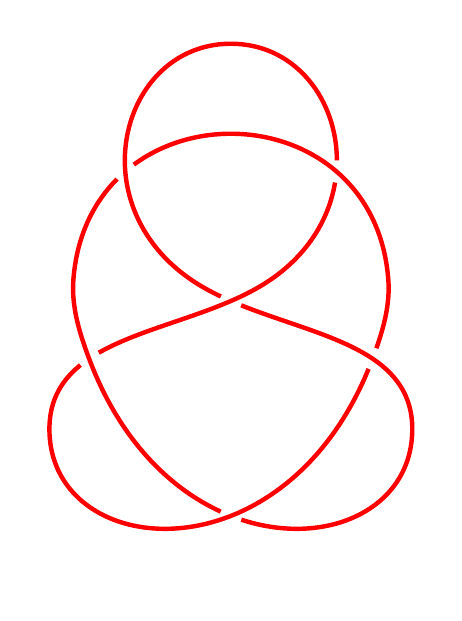
\begin{tikzpicture}
\path[spath/save=6-2] ([closed]2,1) .. (1.8,0) .. (-2.3,-1) .. (.5,1) .. (0,4) .. (-.5,1) .. (2.3,-1) .. (-1.8,0) .. (-2,1) .. (2,1);
\tikzset{spath/knot={6-2}{8pt}{2,4,...,12}}
\end{tikzpicture}
\caption{\(6_2\)}
\autolabel
\end{figure}

\begin{figure}
%% 6_3
\centering
\tikzsetnextfilename{6-3}
%\tikzset{external/export next=false}
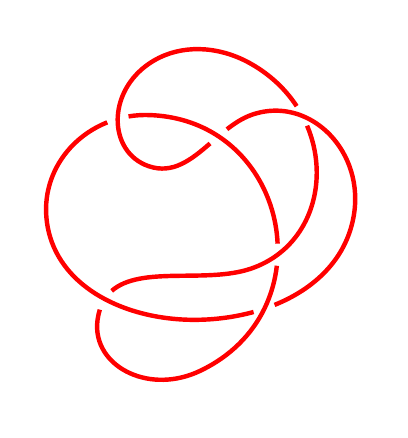
\begin{tikzpicture}
\path[spath/save=6-3,scale=1.3] ([closed]0,0) .. (1.5,1) .. (.5,2) .. (-.5,1.5) .. (-.5,2.5) .. (.5,2.5) .. (.5,.5) .. (-1,0) .. (0,-.5) .. (-.5,2) .. (-1.5,1) .. (0,0);
\tikzset{
  spath/knot={6-3}{8pt}{2,4,...,12}
}
\end{tikzpicture}
\caption{\(6_3\)}
\autolabel
\end{figure}

\begin{figure}
%% 7_1
\centering
\tikzsetnextfilename{7-1}
%\tikzset{external/export next=false}
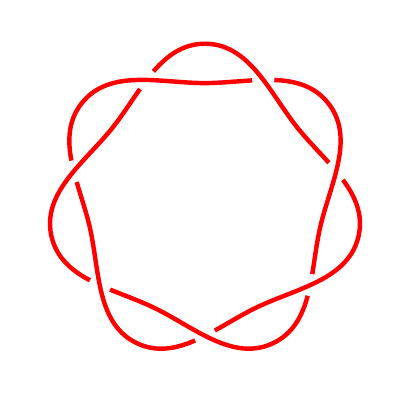
\begin{tikzpicture}
\path[spath/save=7-1] ([closed]90:2) foreach \k in {1,...,7} { .. (90-360/7+\k*720/7:1.5) .. (90+\k*720/7:2) } (90:2);
\tikzset{spath/knot={7-1}{8pt}{2,4,...,14}}
\end{tikzpicture}
\caption{\(7_1\)}
\autolabel
\end{figure}

\begin{figure}
%% 7_2
\centering
\tikzsetnextfilename{7-2}
%\tikzset{external/export next=false}
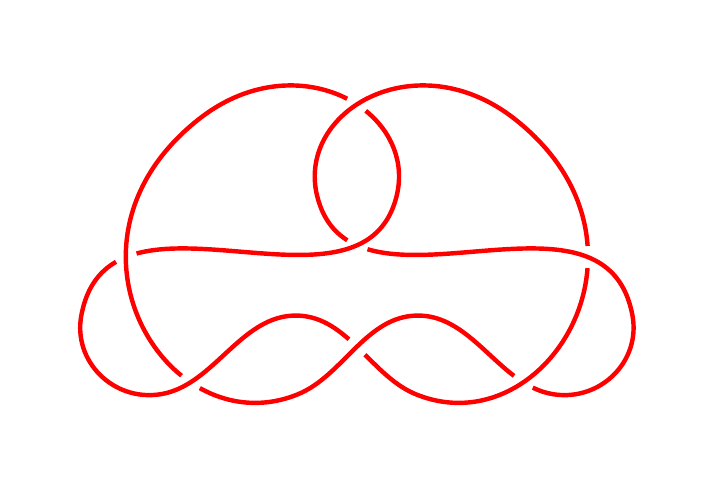
\begin{tikzpicture}
\path[spath/save=7-2] ([closed].75,.5) .. (2.5,-.5) .. (3.5,.5) .. (-.5,2) .. (2,3) .. (.75,-.5) .. (-.75,.5) .. (-2.5,-.5) .. (-3.5,.5) .. (.5,2) .. (-2,3) .. (-.75,-.5);
\tikzset{spath/knot={7-2}{8pt}{2,4,...,14}}
\end{tikzpicture}
\caption{\(7_2\)}
\autolabel
\end{figure}

\begin{figure}
%% 7_3
\centering
\tikzsetnextfilename{7-3}
%\tikzset{external/export next=false}
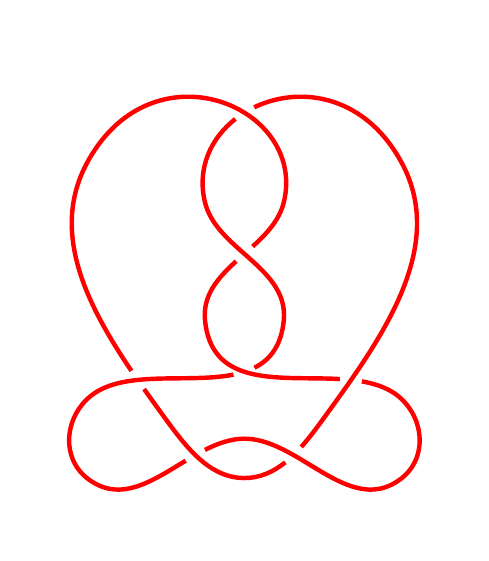
\begin{tikzpicture}
\path[spath/save=7-3] ([closed]0,0) .. (1,.75) .. (2,4) .. (-.5,3.5) .. (.5,2) .. (-2,1) .. (-2,0) .. (0,.5) .. (2,0) .. (2,1) .. (-.5,2) .. (.5,3.5) .. (-2,4) .. (-1,.75);
\tikzset{spath/knot={7-3}{8pt}{2,4,...,14}}
\end{tikzpicture}
\caption{\(7_3\)}
\autolabel
\end{figure}

\begin{figure}
%% 7_4
\centering
\tikzsetnextfilename{7-4}
%\tikzset{external/export next=false}
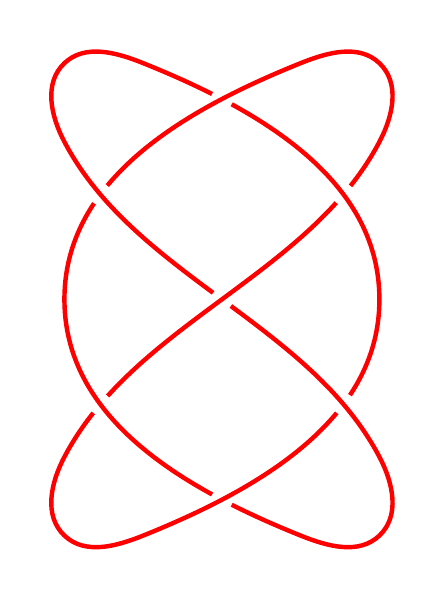
\begin{tikzpicture}
\path[spath/save=7-4] ([closed]-2,2) .. (-2,3) .. (-1,3) .. (2,0) .. (-1,-3) .. (-2,-3) .. (-2,-2) .. (2,2) .. (2,3) .. (1,3) .. (-2,0) .. (1,-3) .. (2,-3) .. (2,-2) .. (-2,2);
\tikzset{spath/knot={7-4}{8pt}{2,4,...,14}}
\end{tikzpicture}
\caption{\(7_4\)}
\autolabel
\end{figure}

\begin{figure}
%% 7_5
\centering
\tikzsetnextfilename{7-5}
%\tikzset{external/export next=false}
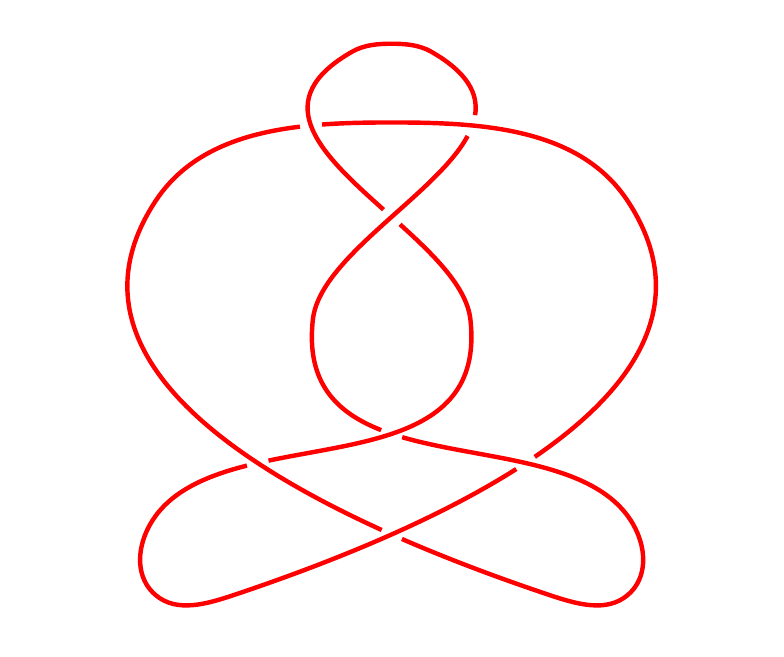
\begin{tikzpicture}
\path[spath/save=7-5] ([closed]0,0) .. (.5,-.1) .. (-1,-3.5) .. (3,-6) .. (3,-7) .. (2,-7) .. (-3,-2) .. (0,-1) .. (3,-2) .. (-2,-7) .. (-3,-7) .. (-3,-6) .. (1,-3.5) .. (-.5,-.1) .. (0,0);
\tikzset{spath/knot={7-5}{8pt}{2,4,...,14}}
\end{tikzpicture}
\caption{\(7_5\)}
\autolabel
\end{figure}

\begin{figure}
%% 7_6
\centering
\tikzsetnextfilename{7-6}
%\tikzset{external/export next=false}
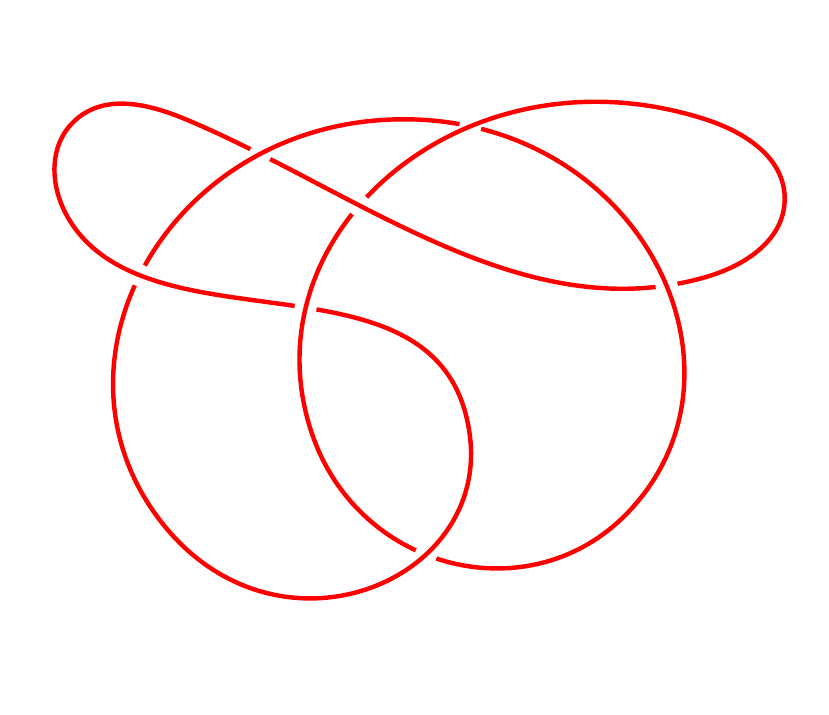
\begin{tikzpicture}
\path[spath/save=7-6] ([closed]0,5) .. (3,0) .. (-1,1) .. (4,5) .. (5,4) .. (4,3) .. (-2.6,5) .. (-4,5) .. (-4,3.6) .. (1,1) .. (-3,0);
\tikzset{spath/knot={7-6}{8pt}{2,4,...,14}}
\end{tikzpicture}
\caption{\(7_6\)}
\autolabel
\end{figure}

\begin{figure}
%% 7_7
\centering
\tikzsetnextfilename{7-7}
%\tikzset{external/export next=false}
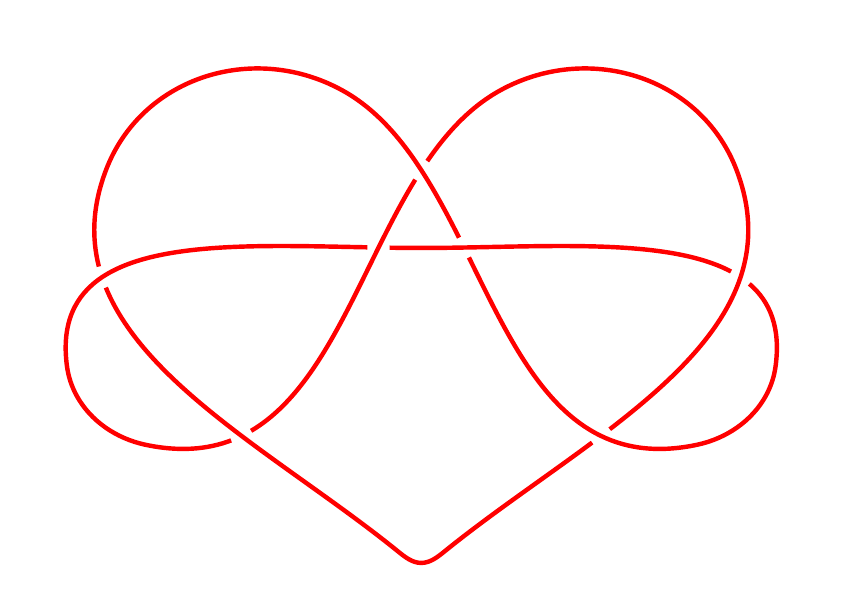
\begin{tikzpicture}
\path[spath/save=7-7] ([closed]3.5,-2.5) .. (4.5,-1.5) .. (0,0) .. (-4.5,-1.5) .. (-3.5,-2.5) .. (1,2) .. (4,1) .. (.3,-3.85) .. (0,-4) .. (-.3,-3.85) .. (-4,1) .. (-1,2);
\tikzset{spath/knot={7-7}{8pt}{2,4,...,14}}
\end{tikzpicture}
\caption{\(7_7\)}
\autolabel
\end{figure}


\end{document}
